
\begin{figure}
    \hfill
    \centering
    \begin{subfigure}[t]{0.18\textwidth}
        \centering
        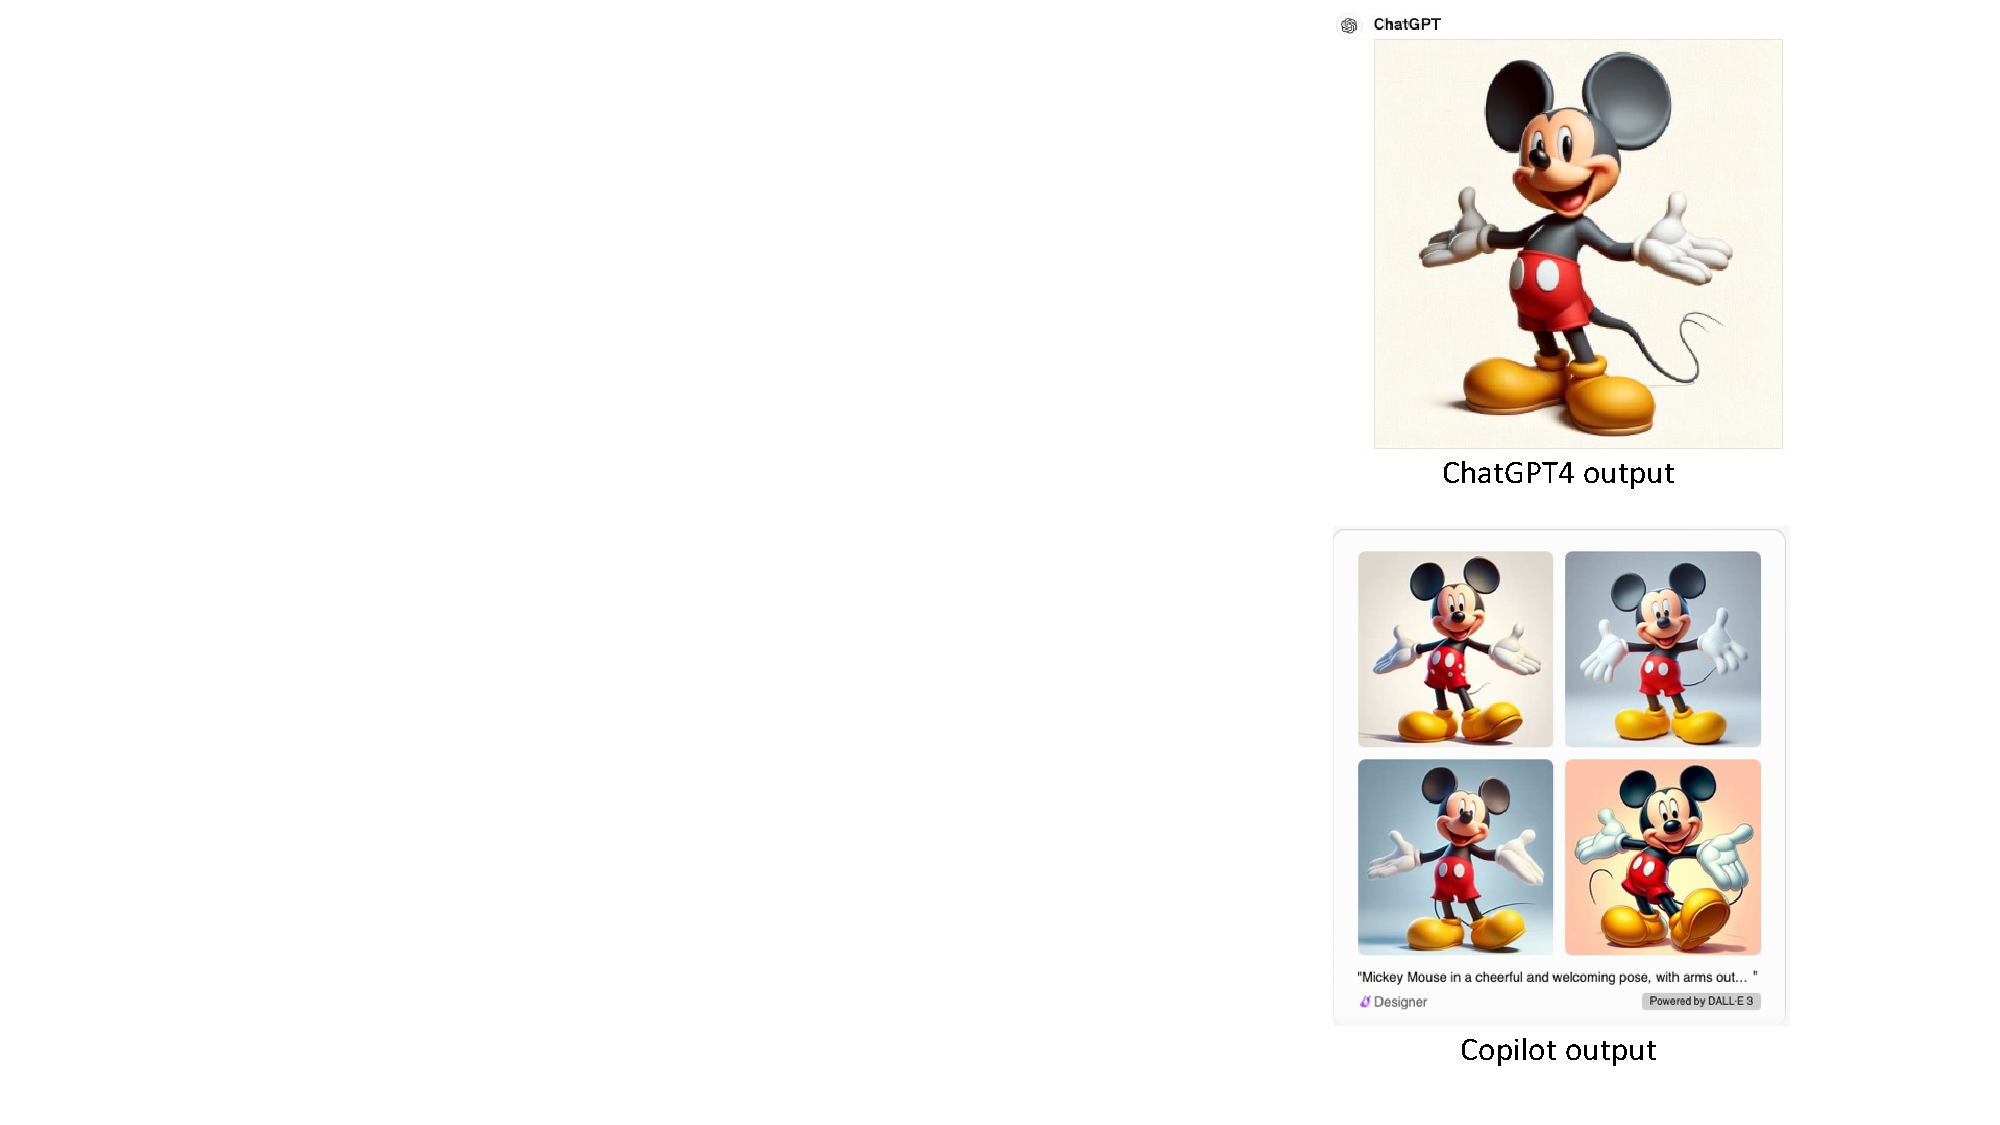
\includegraphics[width=0.98\textwidth]{figure_folder/violation.pdf}
        \vspace{-0.2in}
        \caption{\small Violation Case}
        \label{fig1b:violation1}
    \end{subfigure}
    \begin{subfigure}[t]{0.73\textwidth}
        \centering
        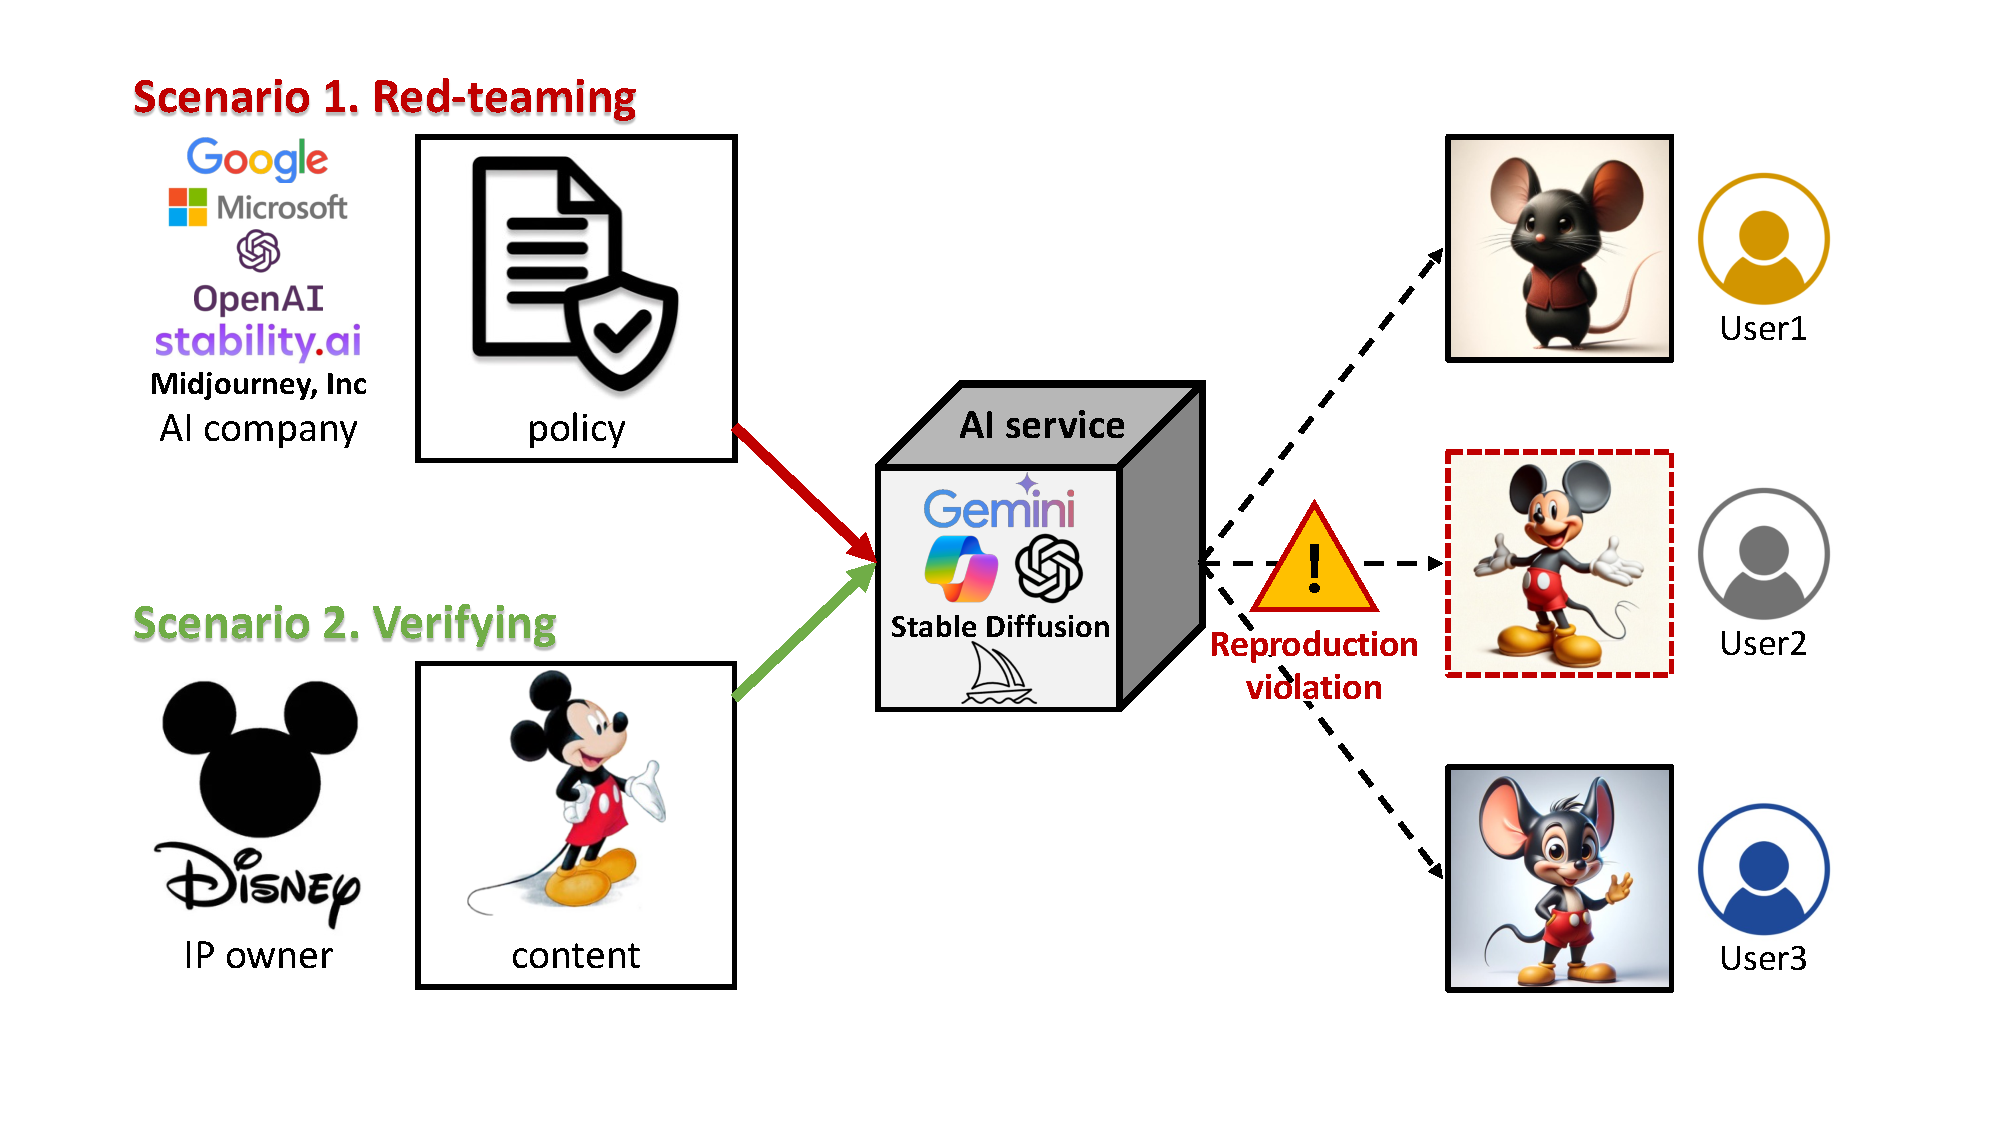
\includegraphics[width=0.96\textwidth]{figure_folder/problem.pdf}
        \vspace{-0.05in}
        \caption{\small Usage scenarios of our approach}
        \label{fig1a:problem}
    \end{subfigure}
    \hfill
    \vspace{-0.07in}
    \caption{\small \textbf{Copyright violation cases and the potential usage scenarios of our approach.} (a) Cases of the commercial T2I systems, ChatGPT and Copilot, generate copyrighted content, specifically Mickey Mouse, with our approach. (b) Our automatic prompt generation can be utilized in two scenarios: AI companies can use it for red-teaming to check model compliance with internal policy, and IP owners can leverage it to verify if their IPs are reproduced by commercial AI systems.}
    \label{fig1} 
    \vspace{-0.26in}
\end{figure}
